\chapter[Operation of segmented detectors in LN$_{2}$]{Operation of segmented detectors in liquid nitrogen}
\label{cha:GII}
Segmented $n$-type germanium detectors will be directly submerged in cryogenic liquid in GERDA Phase II. It is therefore very important to study the performance of segmented detectors in cryogenic liquid. Siegfried~II, the second 18-fold segmented $n$-type prototype detector for GERDA Phase II (see Sec.~\ref{sec:gerda:stat3}) was inserted into the Gerdanlinchen II test stand (see Sec.~\ref{sec:tt:gii}) containing liquid nitrogen on April 23rd, 2008. It was kept in liquid nitrogen for about 5 months and was warmed up on September 15th, 2008. The resolutions and leakage currents of the core and all segments were constantly monitored. Four short cool-down and warm-up cycles were carried out afterward to optimize the setup and perform dedicated measurements. The leakage currents were monitored after each cool-down. The detector performance is summarized in this chapter.

\section{Experimental setup}
\label{sec:gii:setup}
The measurements were performed using the cryogenic test stand, Gerdalinchen~II (GII). A detailed description of GII can be found in Sec.~\ref{sec:tt:gii}.  Figure~\ref{fig:ii:sch} shows the setup of GII for the operation of segmented detectors in liquid nitrogen. The dewar was filled through the filling tube. The numbers inside parentheses indicate the positions of eight PT100 thermal resistors. They were used to monitor the level of the liquid nitrogen. The dewar was refilled once per day to keep the level of liquid nitrogen between PT100 (2) and (3). The infrared shields, hence, were kept inside liquid nitrogen permanently minimizing the infrared radiation load on the detector. There are three mounting positions for detectors. Only the upper and middle ones were used in the measurements.

\begin{figure}[hbtp]
\centering
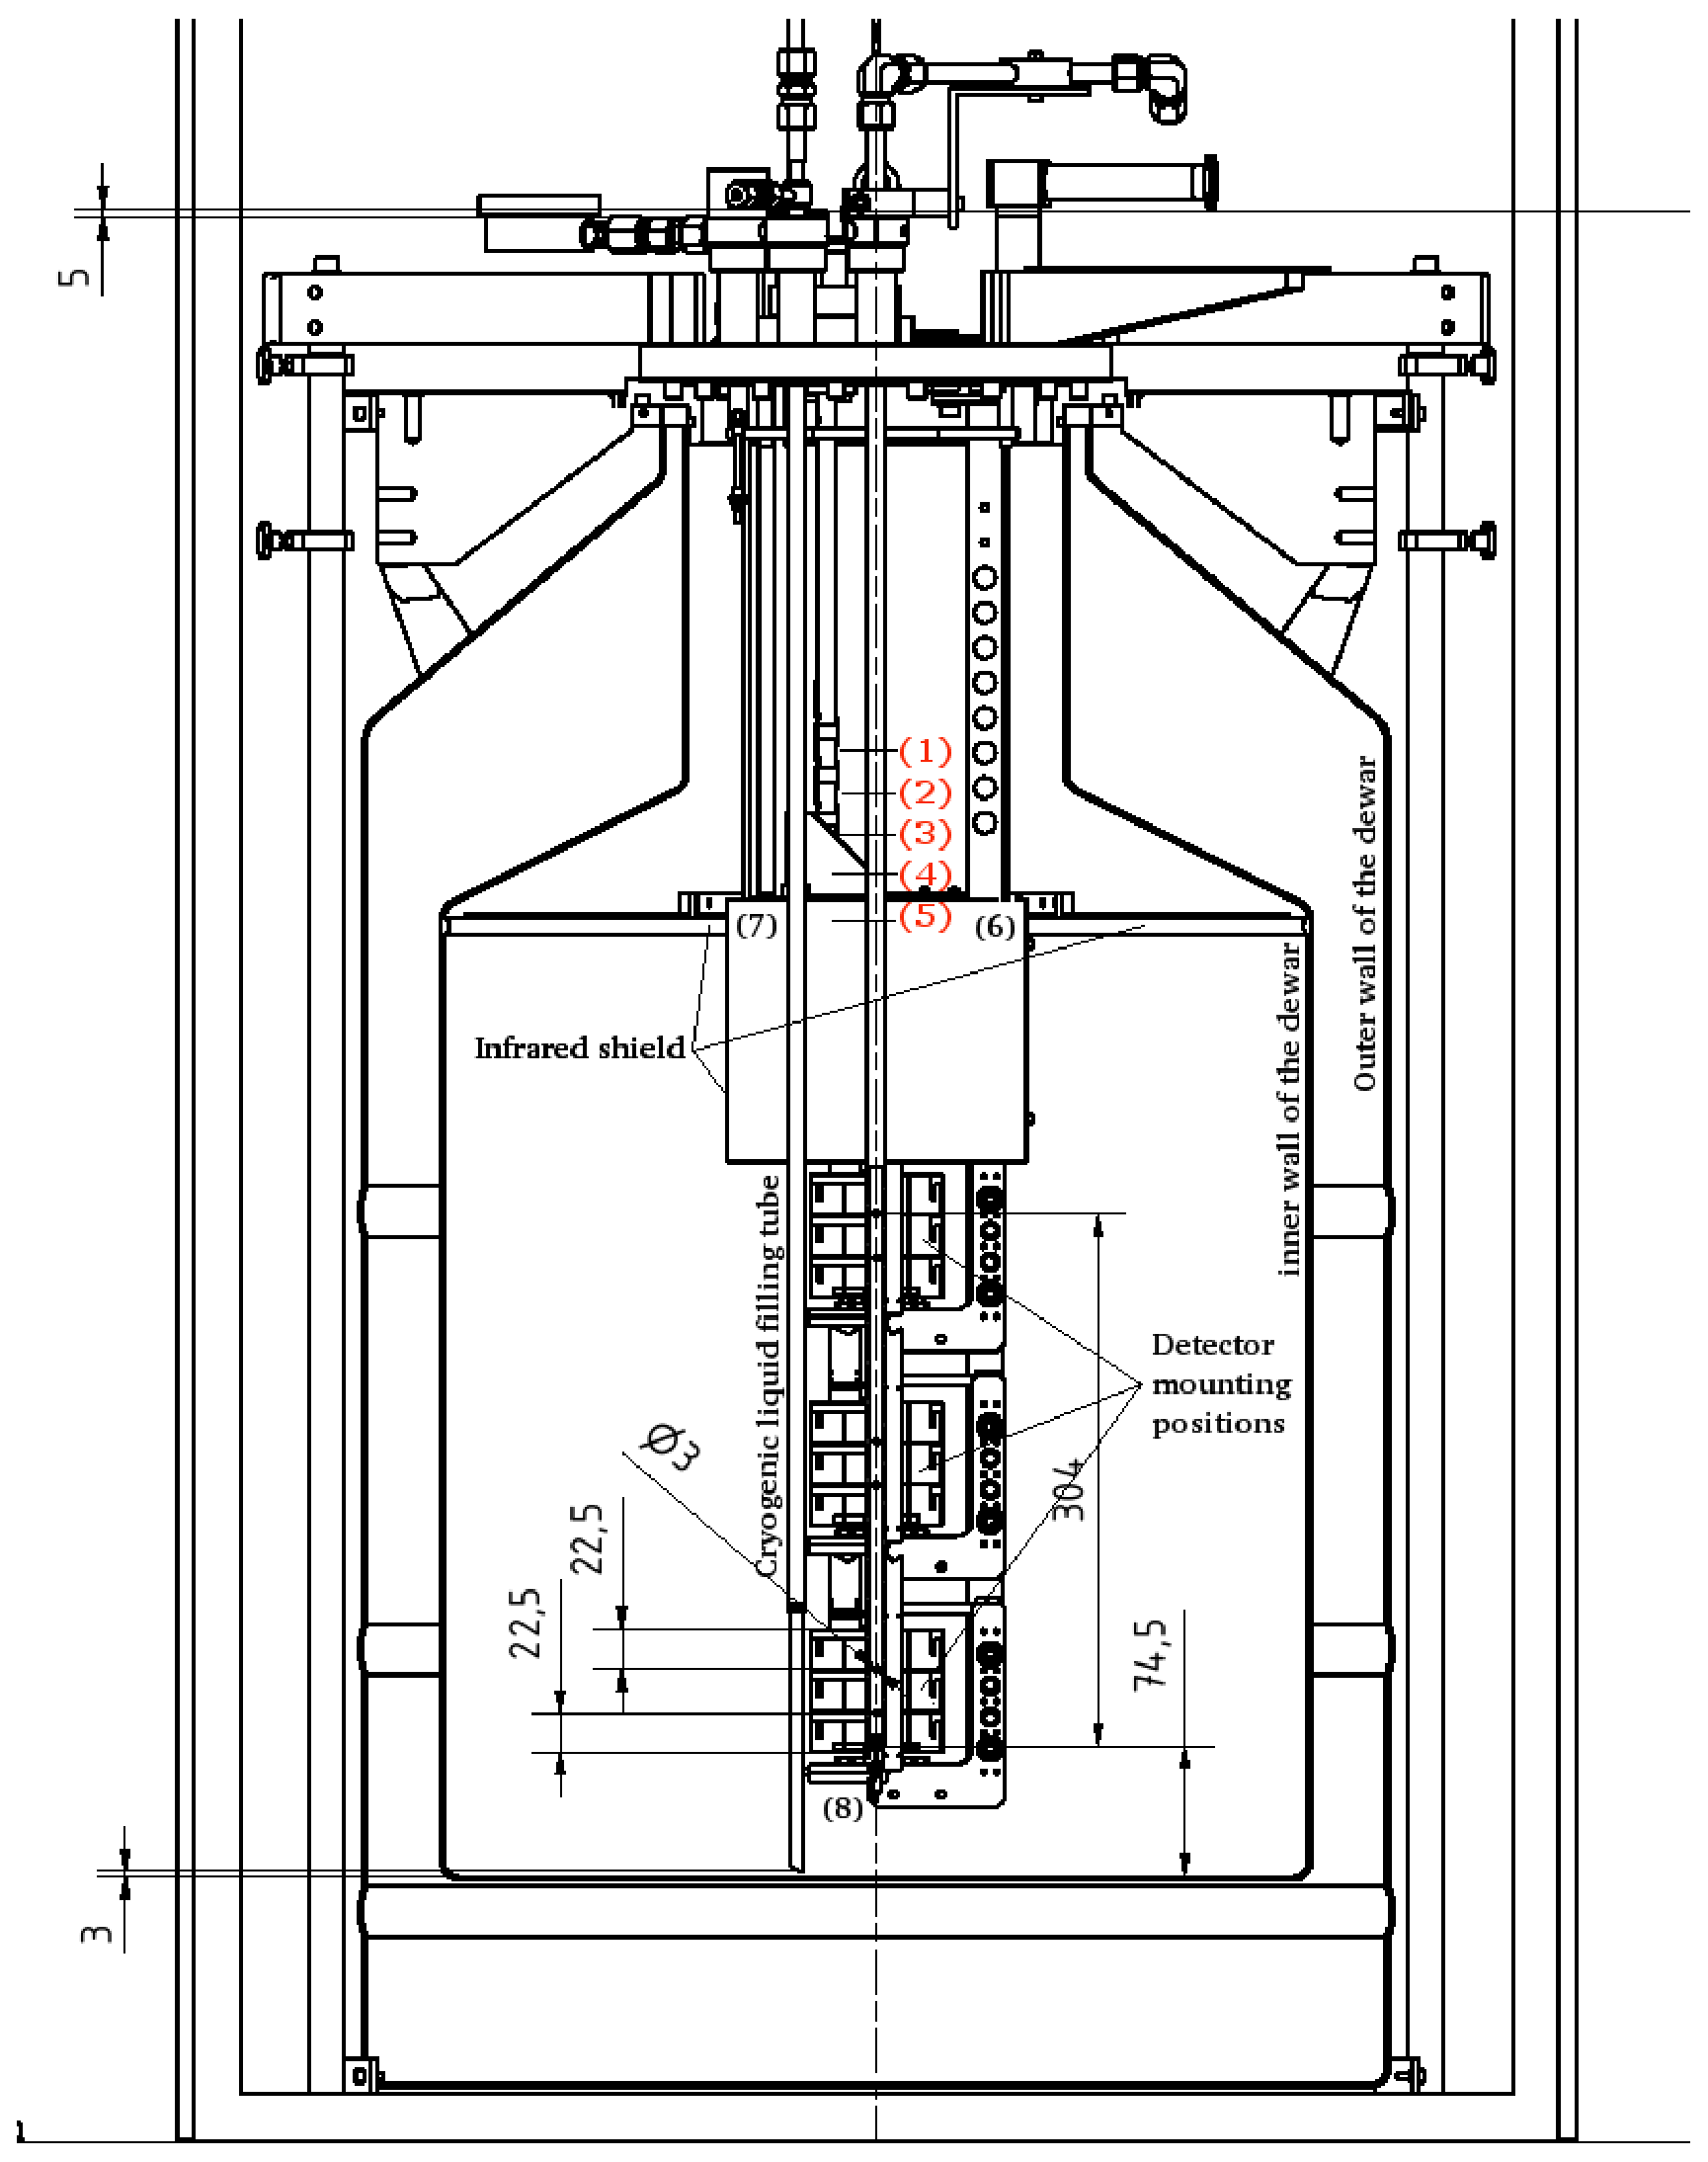
\includegraphics[width=\textwidth]{GIIscheme}
\caption{Gerdalinchen~II setup for the operation of segmented detectors in liquid nitrogen.}
\label{fig:ii:sch}
\end{figure}

\section{Cool-down test}
\label{sec:ii:cool}
The speed, at which the detector strings will be lowered in GERDA, has to be chosen such, that the whole process can be finished in a reasonable time without subjecting the strings and detectors to dangerous thermal and mechanical stress. The submersion speed designed in GERDA is 10~mm/min. The temperature profile of a detector during the submersion process was studied in GII with an aluminum mock-up detector mounted at the highest position as shown in Fig.~\ref{fig:ii:sch}. 

The rising of liquid nitrogen was tuned to be about 10~mm/min. The temperature profile of the mock-up detector was monitored using three PT100 thermal resisters mounted on the top, bottom and in the middle of the mock-up. Figure~\ref{fig:ii:temp} shows the temperature profiles of the mock-up detector during the filling of GII. The thermal sensor 8 was near the bottom of the dewar, and submerged into the liquid immediately after the filling started. The thermal sensor 1 was at the top most position and always above the liquid. The largest temperature difference between the top and bottom  occurred at the first contact of the detector with the liquid nitrogen. It was about $130^{\circ}$C and lasted about three minutes. As germanium has a thermal conductivity four times smaller than aluminum, it is expected that the temperature difference of a germanium detector is four times larger.

\begin{figure}[htbp]
\centering
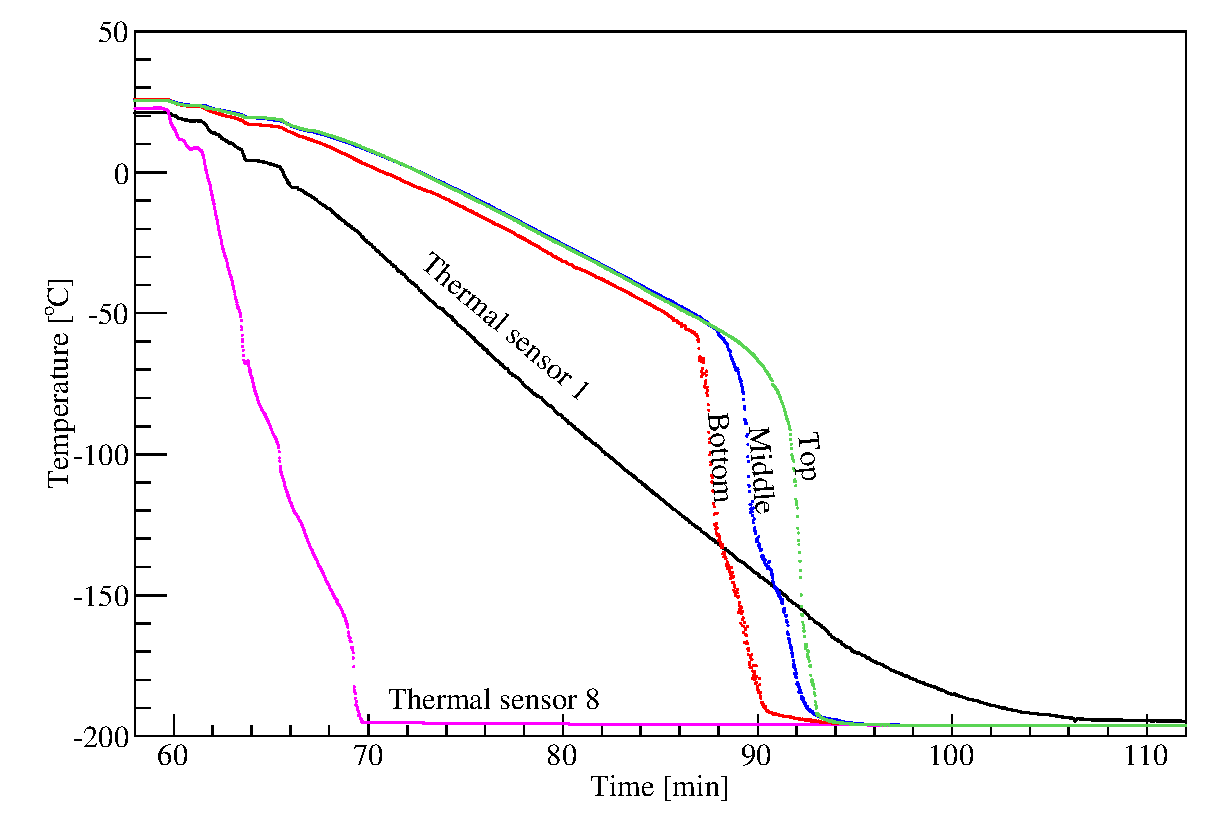
\includegraphics[width=0.8\textwidth]{temp}
\caption{Temperature profiles of a mock-up detector during the cool-down process. GII was filled with liquid nitrogen at the speed of 10~mm/min. The thermal sensor 8 was near the bottom of the dewar, and submerged into the liquid immediately after the filling started. The thermal sensor 1 was at the top most position and always above the liquid. Curves labeled ``Top'', ``Middle'' and ``Bottom'' show the temperature profiles of the mock-up detector.}
\label{fig:ii:temp}
\end{figure}

\section{Resolution}
\label{sec:ii:sigma}
Siegfried II was mounted at the highest position in GII after a detailed cool-down procedure had been developed. It was cooled down on April 23$^{\text{rd}}$, 2008. The core and segment resolutions of Siegfried II were constantly monitored during the 140 days of operation. The variation of the resolutions (FWHM) at 1332~keV is shown for the core in Fig.~\ref{fig:ii:fwhm_core} and for all 18 segments in Fig.~\ref{fig:ii:fwhm_segs}.
\begin{figure}[hbtp]
\centering
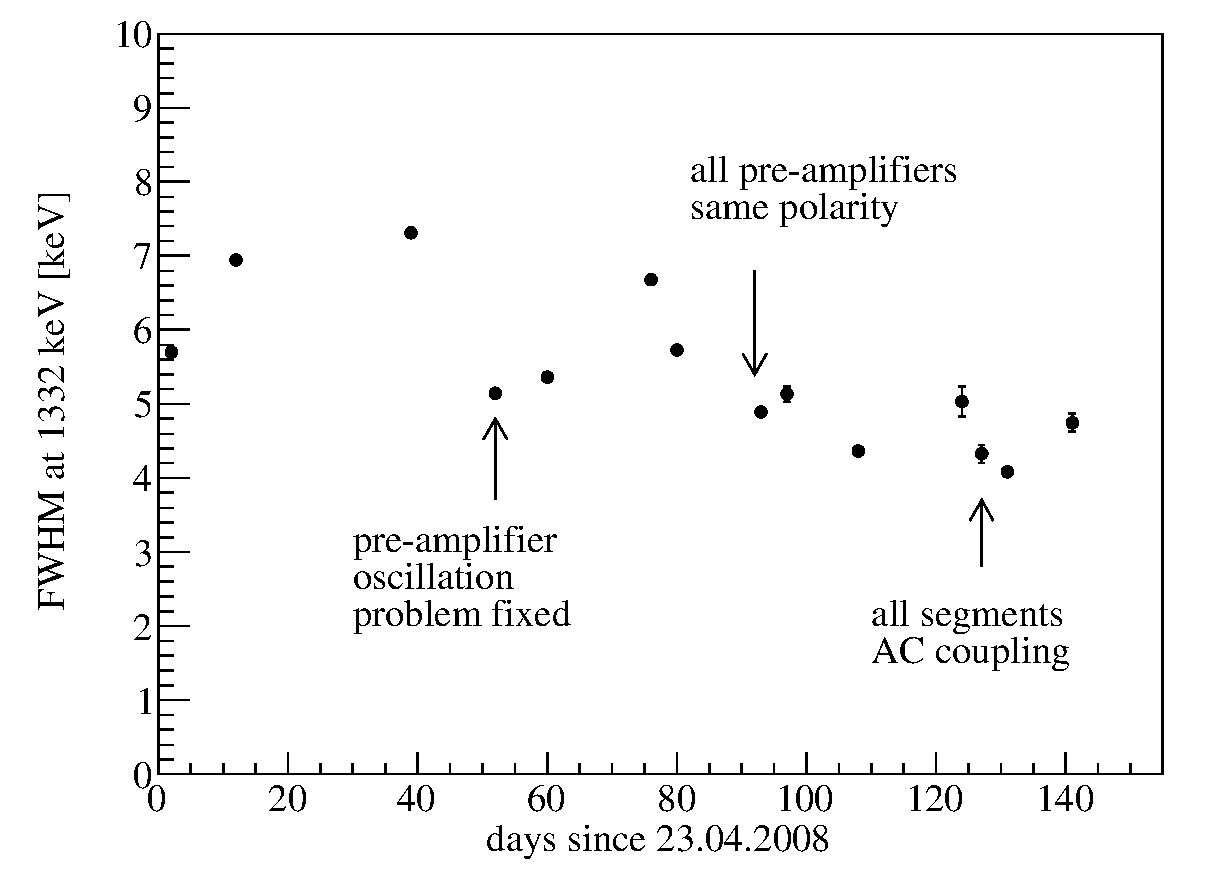
\includegraphics[width=0.6\textwidth]{fwhm_versus_time_core}
\caption{Development of the core resolution of Siegfried II during 140 days of operation. The uncertainties were determined by the fittings of the 1332~keV gamma line. Most of them are smaller than the symbols and cannot be seen on the plot.}
\label{fig:ii:fwhm_core}
\end{figure}

\begin{sidewaysfigure}[tphb]
\centering
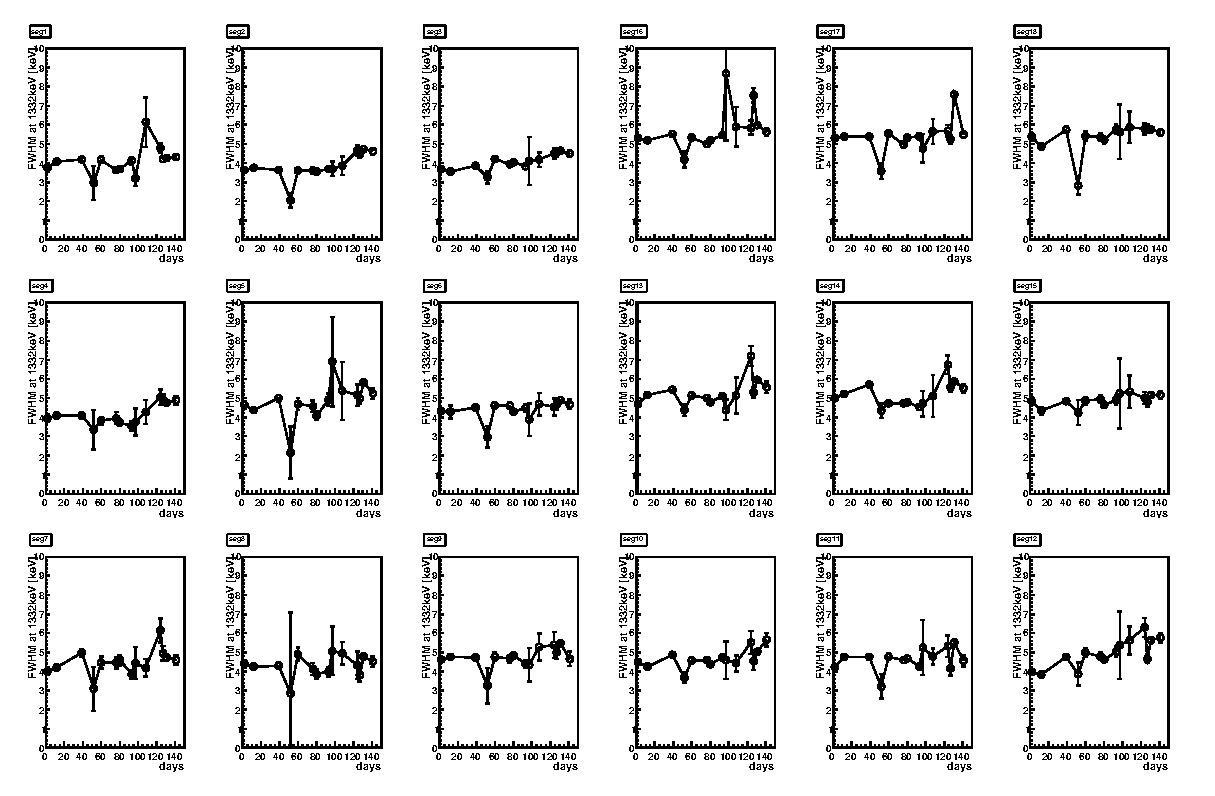
\includegraphics{fwhm_versus_time_segments}
\caption{Development of the segment resolutions of Siegfried II during 140 days of operation. The uncertainties were determined by the fittings of the 1332~keV gamma line. Some of them are smaller than the symbols and cannot be seen on the plot.}
\label{fig:ii:fwhm_segs}
\end{sidewaysfigure}

During the first month of operation, all pre-amplifiers were oscillating whenever all 19 channels were read out simultaneously. The oscillations were due to an insufficient grounding scheme of the copper boxes holding and shielding the pre-amplifiers, see Fig.~\ref{fig:tt:gefb}. The problem was fixed by adding an extra copper plate inside the box, serving as the common ground for all pre-amplifiers. Afterward, all pre-amplifiers could be read out simultaneously and the core resolution was slightly better.

The second problem which affected the core resolution was related to the pulse polarity of the pre-amplifiers. Three pre-amplifiers (segments 3, 15 and 17) had a negative signal polarity while the rest had a positive one. This induced cross talk between these three pre-amplifiers and the core pre-amplifier. Take the 1332~keV photon line as an example, for events with the photon energy deposited inside any of these three segments the energy measured by the core pre-amplifer is about 2~keV smaller than the measured core energy in those events with the same photon energy deposited inside any other segments. These three pre-amplifiers were then replaced, resulting in some improvement in the core resolution as indicated in Fig.~\ref{fig:ii:fwhm_core}.

In order to decouple the segment potentials from the pre-amplifiers, all segment were DC instead of AC coupled ten days before the first warm-up, using 1~G$\Omega$ resistors and 2.2~nF capacitors. This improved slightly the core resolution, but not those of the segments.


\section{Leakage current}
\label{sec:ii:current}
The leakage current of Siegfried~II at 2000~V was constantly monitored during the 140 days of operation. Two measurement methods were used: (a) direct measurement with a peco-ampmeter and (b) indirect measurement by comparing the baselines at 0~V and 2000~V. The results from both methods are shown in Fig.~\ref{fig:ii:lc}. The leakage current stayed constant, around 20~pA.

\begin{figure}[htbp]
\centering
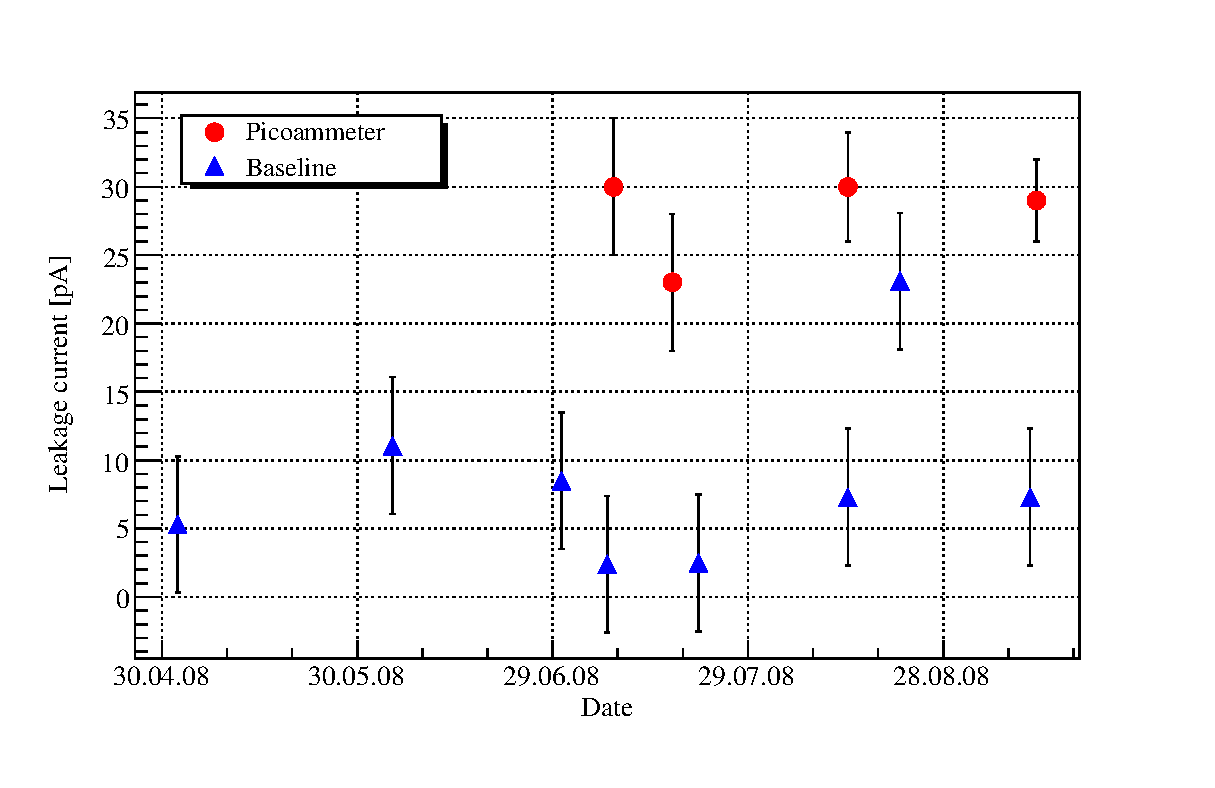
\includegraphics[width=0.6\textwidth, clip]{LC}
\caption{Leakage current of Siegfried II at 2000~V. Two different measurement methods were used. The first was to use a peco-ampmeter to directly measure the leakage current at 2000~V. The second was to compare the baselines at 0~V and 2000~V.}
\label{fig:ii:lc}
\end{figure}

Siegfried~I was mounted at the middle position in GII after the first warm-up of Siegfried~II. Afterward, four cool-down and warm-up cycle were performed. Leakage currents of Siegfried I and II at operation voltage after each cool-down are shown in Fig.~\ref{fig:ii:lcs1} and \ref{fig:ii:lcs2}, respectively. The immediate measurements after each cool-down showed a dramatic increase of the leakage current. However, the leakage current kept dropping until reaching a constant value within around 40 minutes after the cool-down. The measurements after that showed no increase of leakage current for Siegfried~II. This indicates some increase of the capacitance of the contacts between the detector surfaces and the signal cables. The cable connecting Siegfried~II had a permanent failure during the insertion of a gamma source into the core of the detector.

\begin{figure}[htbp]
\centering
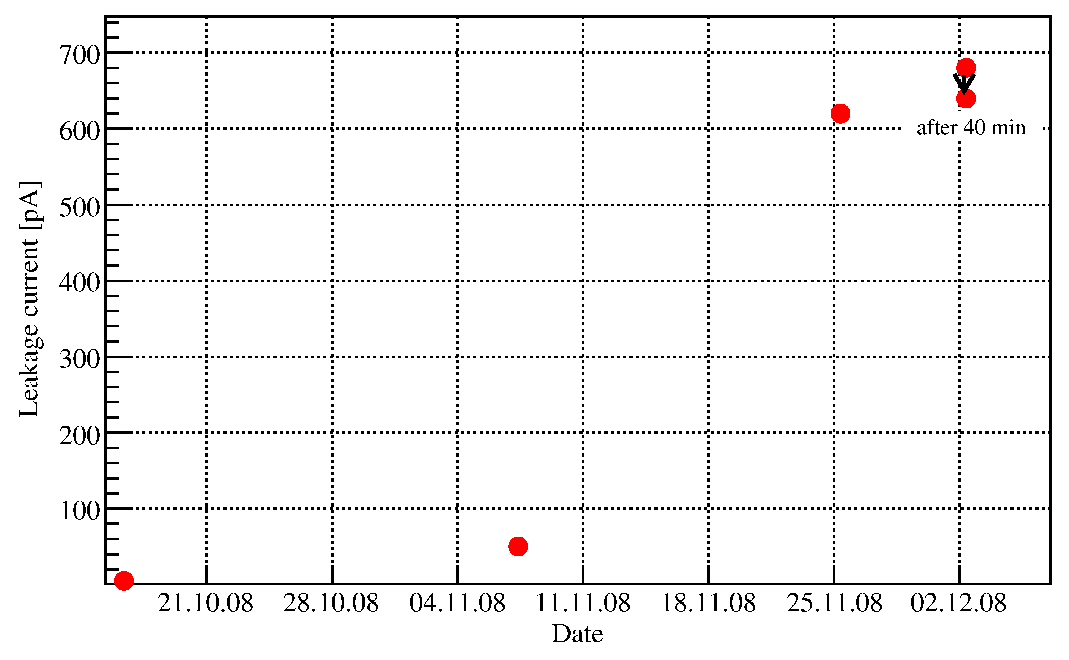
\includegraphics[width=0.6\textwidth]{LCs1}
\caption{Leakage current of Siegfried I at 3000~V right after each cool-down. The currents were measured directly using a peco-ampmeter.}
\label{fig:ii:lcs1}
\end{figure}

\begin{figure}[htbp]
\centering
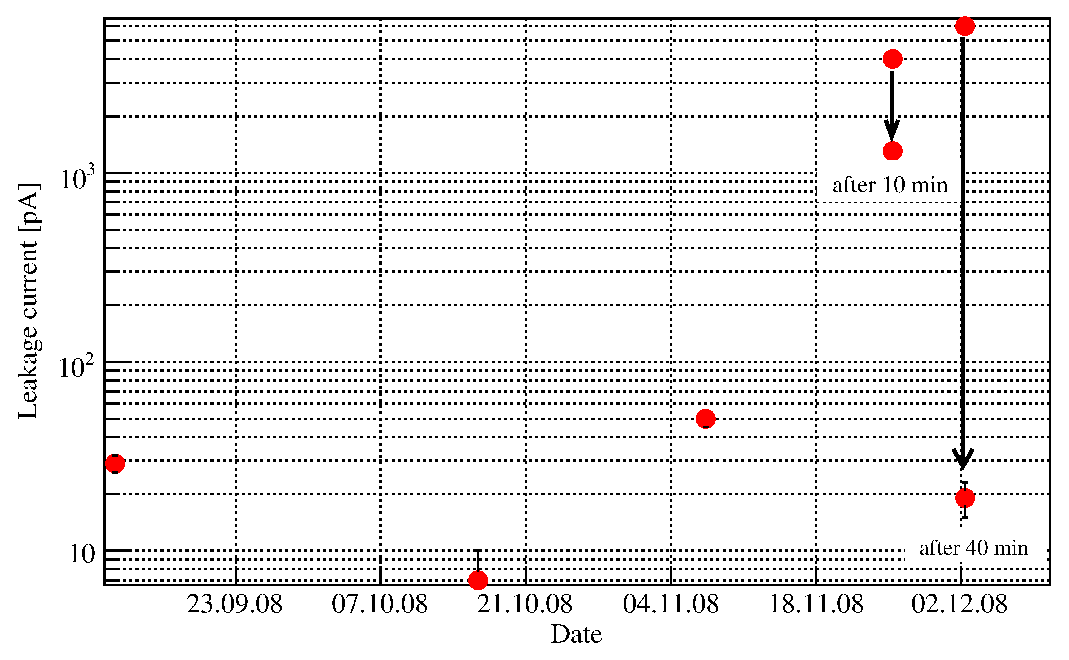
\includegraphics[width=0.6\textwidth, clip]{LCs2}
\caption{Leakage current of Siegfried II at 2000~V after each cool-down. The currents were measured directly using a peco-ampmeter.}
\label{fig:ii:lcs2}
\end{figure}

% \section{Capacitance measurement}
% \label{sec:ii:c}

% \section{Cross talk}
% \label{sec:ii:xtalk}
% with siegfried-II mounted.  The HV cable was connected through the HV feedthrough built on the top flange.  The shield of the HV cable was connected to the top flange.  Under the flange (thus inside the dewar) non-shielded Habia cable (?) was used for both the HV cable and the signal cables for the 18 segments.  A 2.2~nF capacitor and 1~G$\Omega$ resistor were used for the HV filter.  Another 2.2~nF capacitor was used for the core AC coupling. The two capacitors and the resistor were positioned right below the top flange, thus not inside the liquid Nitrogen and only in the gas Nitrogen enviroument.

\section{Negative pulse}
\label{sec:ii:npulse}
The pre-amplifiers and the DAQ system were configured such, that all the channels had positive polarity, \textit{i.e.}, the signals were positive pulses. About 10\% of the events nevertheless had negative pulses in some of the segments. Figure~\ref{fig:ii:npul} shows a typical negtive pulse event. In this single-segment event all the energy was deposited in segment 2. Both segment 1 and 3 showed a transient pulse, \textit{i.e.}, some disturbance of the baseline. The baseline in the segment 3, however, remained shifted. The DAQ should translates this into a negative energy, but actually set the value to zero.

\begin{sidewaysfigure}[htbp]
\centering
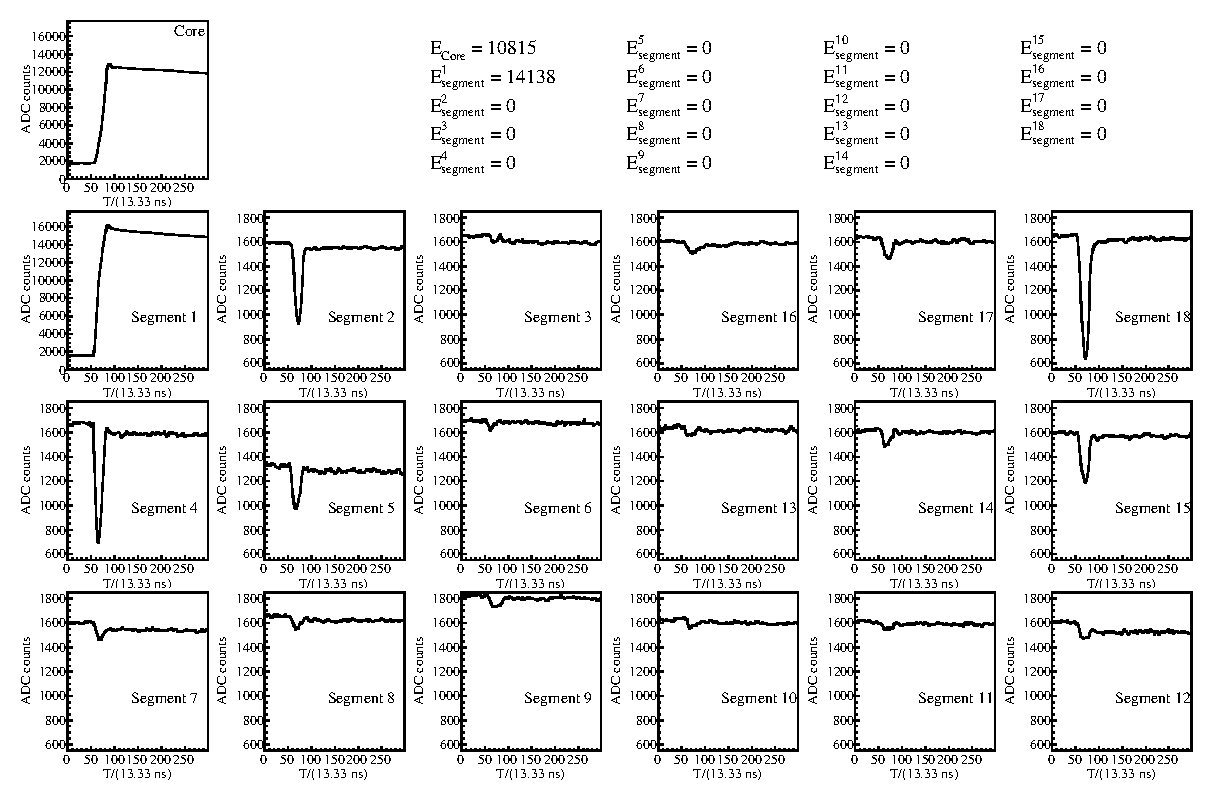
\includegraphics{npul}
\caption{An event showing a negative baseline shift in segment 3. Both segment 1 and 3 show baseline disturbances, but in segment 1 the baseline returns to its original level.}
\label{fig:ii:npul}
\end{sidewaysfigure}

\subsection{Selection of negative pulse events}
\label{sec:ii:frac}
The sum of the energies seen in all segments, $\sum E_{\text{segment}}$, (including negative energies) agrees with the core energy, $E_{\text{core}}$, within the resolution. However, since the DAQ system estimated the energy of a negative pulse to be zero (as for the event depicted in Fig.~\ref{fig:ii:npul}), the sum of the segment energies as calculated by DAQ, $\sum E^{\text{DAQ}}_{\text{segment}}$, was larger than $E_{\text{core}}$. By comparing  $\sum E^{\text{DAQ}}_{\text{segment}}$ and $E_{\text{core}}$, negative pulse events were identified and selected.

Figure~\ref{fig:ii:sEnegPulse} shows $\sum E^{\text{DAQ}}_{\text{segment}}$ versus $E_{\text{core}}$ of a data sample collected with a $^{228}$Th source mounted inside GII on top of Siegfried II. The two solid lines in the plot indicate the $\pm 20 \sigma$ range around the core energy. Points above the upper solid line correspond to the events with negative baseline shift. There is also a very small fraction of events with$\sum E^{\text{DAQ}}_{\text{segment}} < E_{\text{core}}$. This is due to noise or pile-up\footnote{Two pulses are too close to each other in time for DAQ to get a correct estimation of energy.} effects. The fraction of the events with negative baseline shift is about 10\%.

\begin{figure}[tphb]
\centering
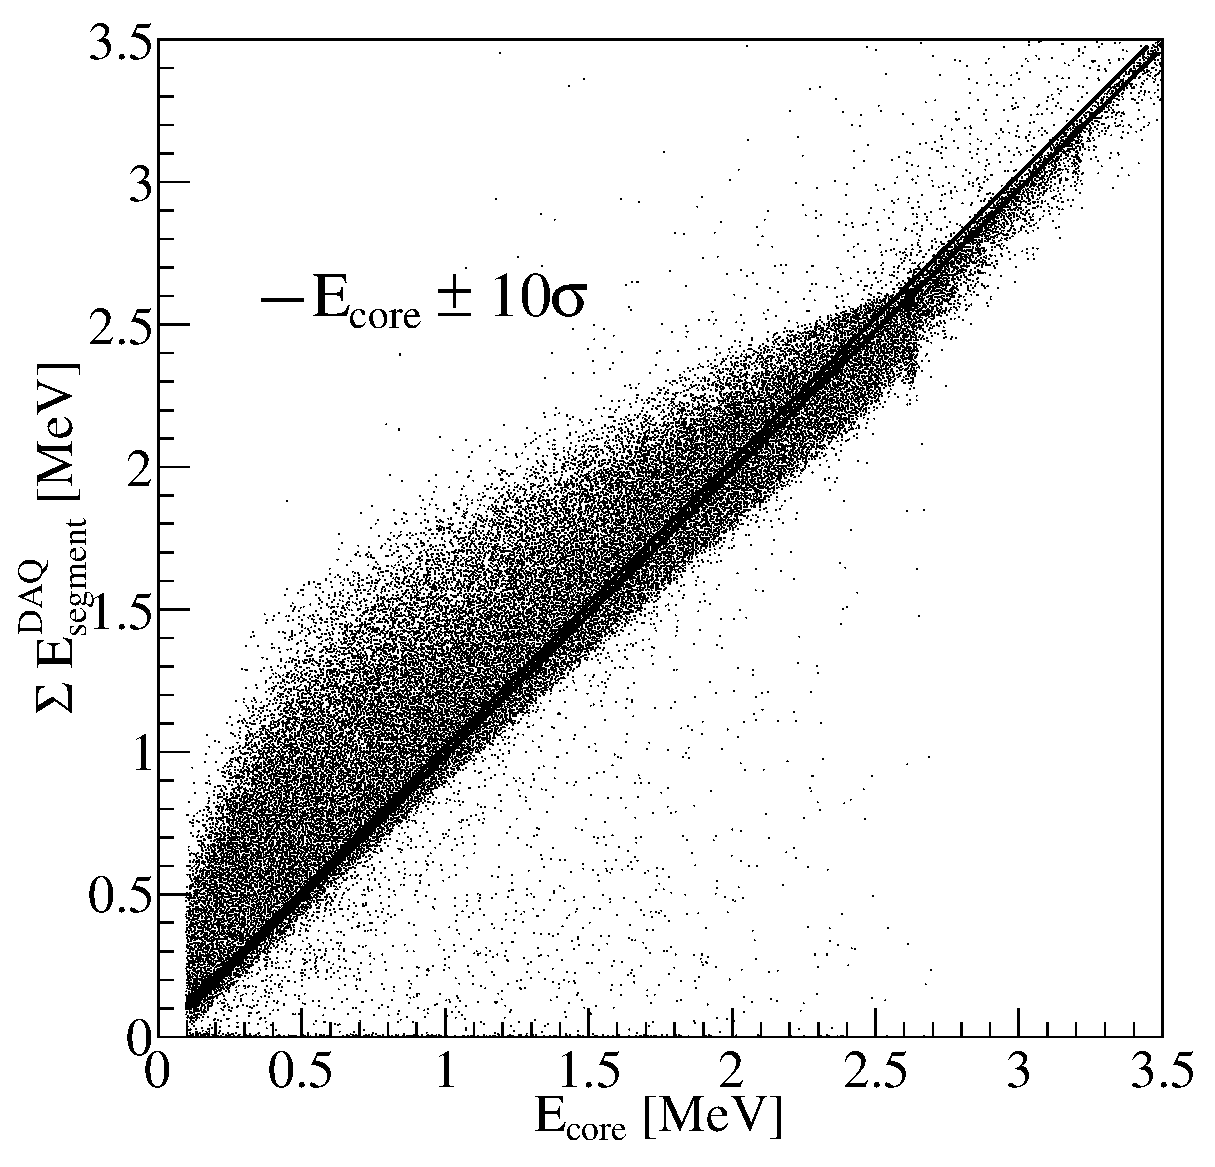
\includegraphics[width=0.5\textwidth]{sEnegPuls}
\caption{Sum of energies from all segments versus the core energy. All energies were calculated by the DAQ system. The two solid lines indicate the 20$\sigma$ range of the core energy.}
\label{fig:ii:sEnegPulse}
\end{figure}

\subsection{Location of negative baseline shifts}
\label{s:locneg}
To figure out whether the negative baseline shifts predominatly occur in special segments, the energies from individual segments were plotted versus the core energy as shown in Fig.~\ref{f:ii:EnegPulse}. Negative pulse events were featured with  $E_{\text{segments}} > E_{\text{core}}$. They mainly populated in the segments on the top and bottom of the detector. Very few negative pulse events were found in the segments in the middle of the detector.

\begin{sidewaysfigure}[tphb]
\centering
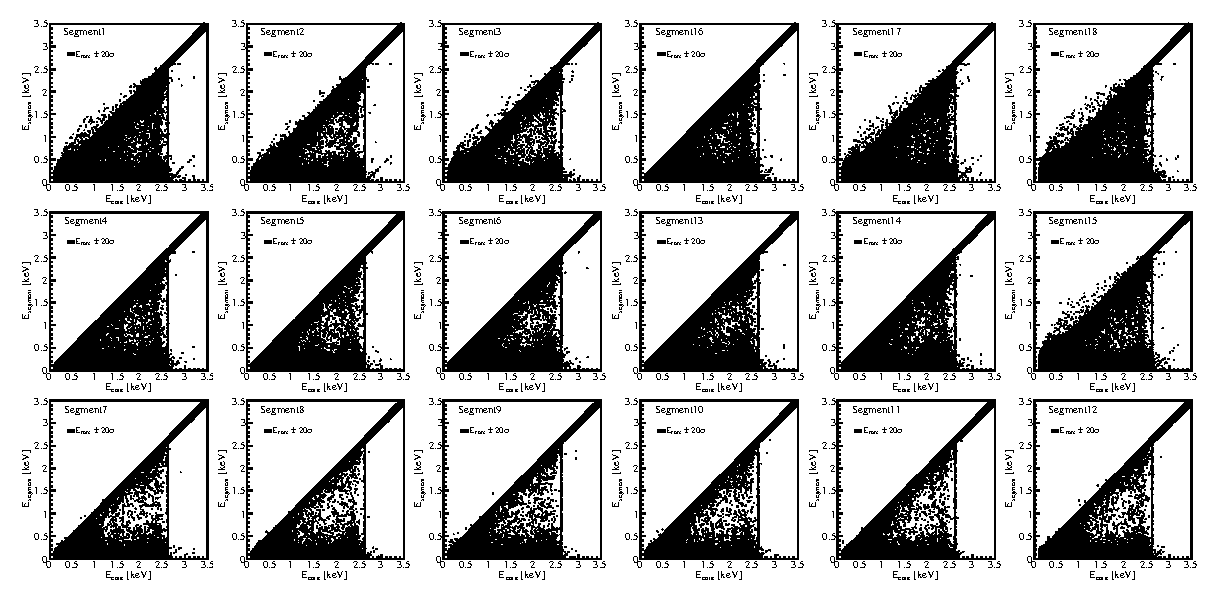
\includegraphics{EnegPuls}
\caption{Energies of individual segments versus the core energy. All energies were calculated by the DAQ system. The two solid lines in each plot indicate the $\pm 20 \sigma$ range around the core energy.}
\label{f:ii:EnegPulse}
\end{sidewaysfigure}

\subsection{Possible explanation}
\label{s:ii:exp}
The fact that the negative baseline shifts occur predominantly in the top and bottom segments of the detector indicates that there might be surface channels~\cite{Sur05} formed, where the electric field was distorted and the rise time of the pulse increased subsequently. The DAQ energy filter could not handle the pulse with long rise time correctly and give an energy slightly smaller than the full energy. This would enhance the event rate on the low energy side of a full-energy peak at the cost of the peak itself. This was seen in Fig.~\ref{fig:ph:mca}: the low energy side of the 1332~keV peak in data is significantly higher than that in simulation in which the surface channel effect was not taken into account.

However, if the assumption were true, the fraction of negative pulse events in the low energy photon peaks should be larger than in high energy photon peaks, because low energy photons deposit their energies in average closer to the detector surface than photons with higher energies. Events within six photon peaks from the $^{228}$Th energy spectrum were selected to examine the assumption. They are 239~keV from $^{212}$Pb, 583~keV from $^{208}$Tl, 861~keV from $^{208}$Tl, 2615~keV from $^{208}$Tl and its double- and single-escape peak 1592~keV and 2103~keV. For each of these 6 sub data samples the fractions of events with $\sum E_{\text{segment}} - E_{\text{core}} \gtrsim 20\sigma$ were calculated and plotted as a function of the core energy, as shown in Fig.~\ref{f:fnp_e}. No obvious correlation was found. This does not support the assumption. 

\begin{figure}[tphb]
\centering
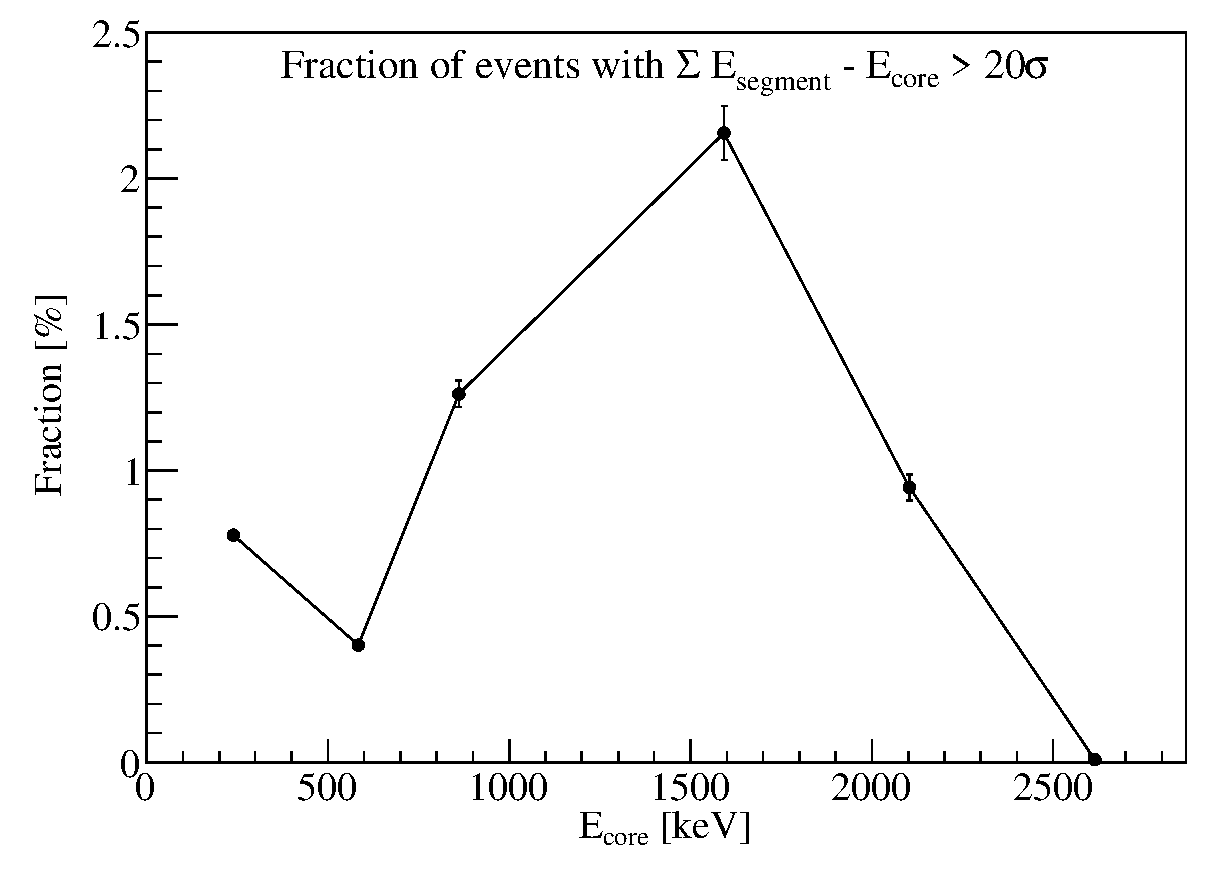
\includegraphics[width=0.6\textwidth]{fnp_e}
\caption{Fraction of events with $\sum E_{\text{segment}} - E_{\text{core}} \gtrsim 20\sigma$ as a function of core energy. The error bars indicate the statistic uncertainty.}
\label{f:fnp_e}
\end{figure}

\section{Summary}
\label{sec:ii:sum}
A long term operation of Siegfried~II submerged in liquid nitrogen was performed using GII. Main performance parameters, such as resolution and leakage current, etc., were constantly monitored. Siegfried~I was inserted into GII after the first warm-up of Siegfried~II. They went through four cool-down and warm-up cycles together. No obvious decrease of the performance was found. A small fraction of events taken with this setup had segments with negative baseline shifts which also affected the core energy. The phenomenon is not yet understood.


%%% Local Variables:
%%% mode:latex
%%% TeX-master: "thesis"
%%% End:
